\documentclass[12pt,a4paper]{article}
\usepackage[margin=1in]{geometry}
\usepackage{amsmath}
\usepackage{amsfonts}
\usepackage{amssymb}
\usepackage{enumitem}
\usepackage{fancyhdr}
\usepackage{titlesec}
\usepackage{array}
\usepackage{longtable}

\usepackage{amsmath}
\usepackage{tikz}

% Header and footer setup
\pagestyle{fancy}
\fancyhf{}
\fancyhead[C]{\textbf{Graduate Aptitude Test in Engineering}}
\fancyfoot[C]{\thepage}

% Section title formatting
\titleformat{\section}{\large\bfseries}{\thesection}{1em}{}
\titleformat{\subsection}{\normalsize\bfseries}{\thesubsection}{1em}{}

\begin{document}

% Title page information
\begin{center}
{\LARGE \textbf{Graduate Aptitude Test in Engineering}}\\[0.5cm]
{\Large \textbf{AE: AEROSPACE ENGINEERING}}\\[0.3cm]
{\large 1st Feb shift 2}\\[0.5cm]

\begin{tabular}{|l|l|}
\hline
\textbf{Total Questions:} & 65 \\
\hline
\textbf{Total Marks:} & 100.0 \\
\hline
\end{tabular}
\end{center}

\vspace{1cm}



% Section A - General Aptitude
\section*{SECTION A - GENERAL APTITUDE}
\begin{center}
\begin{tabular}{|l|l|}
\hline
\textbf{Number of Questions:} & 10 \\
\hline
\textbf{Section Marks:} & 15.0 \\
\hline
\end{tabular}
\end{center}

\subsection*{Question 1 [MCQ]}
Choose the appropriate word/phrase, out of the four options given below, to complete the following sentence:
\begin{enumerate}[label=(\alph*)]
\item harbours
\item leads to  
\item supports
\item affects
\end{enumerate}

\subsection*{Question 2 [MCQ]}
Fill in the blank with the correct idiom/phrase:
That boy from the town was a \_\_\_\_ in the sleepy village.
 
\begin{enumerate}[label=(\alph*)]
\item dog out of herd
\item sheep from heep
\item fish out of water
\item bird from the flock
\end{enumerate}

\subsection*{Question 3 [MCQ]}
Choose the statement where the underlined word is used correctly: 
Apparent lifelessness \_\_\_\_ dormant life.
\begin{enumerate}[label=(\alph*)]
\item When the teacher eludes to different authors, he is being elusive.
\item When the thief keeps eluding the police, he is being elusive 
\item Matters that are difficult to understand, identify or remember are allusive.
\item Mirages can be allusive, but a better way to express them is illusory.
\end{enumerate}

\subsection*{Question 4 [MCQ]}
Tanya is older than Eric.
Cliff is older than Tanya.
Eric is older than Cliff.
If the first two statements are true, then the third statement is:
\begin{enumerate}[label=(\alph*)]
\item True
\item false  
\item uncertain
\item data insufficient
\end{enumerate}

\subsection*{Question 5 [MCQ]}Five teams have to compete in a league, with every team playing every other team exactly once, before going to the next round. How many matches will have to be held to complete the league round of matches?

\begin{enumerate}[label=(\alph*)]
\item 20
\item 10  
\item 8
\item 5
\end{enumerate}

\subsection*{Question 6 [MCQ]}
Select the appropriate option in place of underlined part of the sentence.
\underline{Increased productivity necessary}reflects greater efforts made by the employees.
\begin{enumerate}[label=(\alph*)]
\item Increase in productivity necessary
\item Increase productivity is necessary 
\item Increase in productivity necessarily
\item No improvement required
\end{enumerate}

\subsection*{Question 7 [MCQ]}
Given below are two statements followed by two conclusions. Assuming these statements to be true, decide which one logically follows.

\textbf{Statements:}
I. No manager is a leader.
II. All leaders are executives.

\textbf{Conclusions:}
I. No manager is an executive.
II. No executive is a manager.
\begin{enumerate}[label=(\alph*)]
\item Only conclusion I follows
\item Only conclusionII follows
\item Neither conclusion I nor II follows 
\item Both conclusions I and II follow
\end{enumerate}



\subsection*{Question 8 [NAT]}
\vspace{0.3cm}

In the given figure angle \( Q \) is a right angle, \( PS:QS = 3:1 \), \( RT:QT = 5:2 \), and \( PU:UR = 1:1 \). If the area of triangle \( QTS \) is \( 20 \, \text{cm}^2 \), then the area of triangle \( PQR \) in \( \text{cm}^2 \) is \_\_\_\_.

\vspace{0.5cm}

\begin{center}
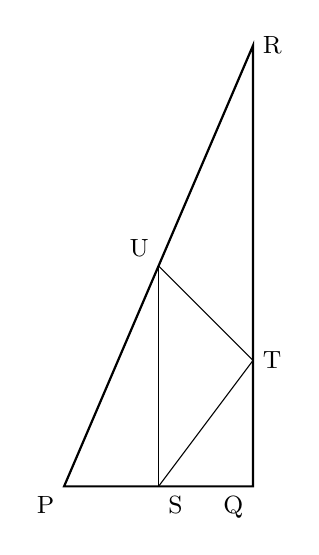
\begin{tikzpicture}[scale=0.8]
    % Coordinates reflecting PS:QS = 3:1, RT:QT = 5:2, PU:UR = 1:1
    \coordinate (Q) at (0,0);                  % Origin
    \coordinate (S) at (-1.5,0);                % QS = 1 unit, PS = 3 units
    \coordinate (P) at (-3,0);                 % So PS = 3 units
    \coordinate (T) at (0,2);                % QT = 2 units
    \coordinate (R) at (0,7);                % RT = 5 units => RT:QT = 5:2
    \coordinate (U) at (-1.5,3.5);            % Midpoint of PR

    % Triangle edges
    \draw[thick] (P) -- (Q) -- (R) -- cycle;
    \draw (P) -- (S);
    \draw (S) -- (Q);
    \draw (R) -- (T);
    \draw (T) -- (Q);
    \draw (P) -- (U) -- (R);
    \draw (U) -- (T);
    \draw (U) -- (S);
    \draw (S) -- (T);

    % Labels
    \node[below left] at (Q) {\small Q};
    \node[below right] at (S) {\small S};
    \node[right] at (T) {\small T};
    \node[right] at (R) {\small R};
    \node[above left] at (U) {\small U};
    \node[below left] at (P) {\small P};
\end{tikzpicture}
\end{center}




\subsection*{Question 9 [MCQ]}
Right triangle PQR lies in the xy-plane so that the right angle is at point P(0, 0) and line PR is parallel to the x-axis. The coordinates of Q are (0, 4). If the coordinates of R are such that the triangle’s area is 30, and S is 3 and 5 is 30. How many different triangles could be constructed with these properties?

\begin{enumerate}[label=(\alph*)]
\item 119
\item 1100  
\item 9900
\item 19800
\end{enumerate}


\subsection*{Question 10 [MCQ]}
There are 3 boxes. Let x be the word that occurs in each of the first two boxes. Let y be the word that occurs in the second and third box. Let z be the word that occurs in these boxes but not in combination with the other in any of the three boxes. Then:
\begin{enumerate}[label=(\alph*)]
\item x,y and z are independent
\item  x and z are independent
\item y and z are independent
\item x and y are independent
\end{enumerate}



\subsection*{Question 11 [MCQ]}
The equation is $\frac{\partial^2 u}{\partial x^2} + \frac{\partial^2 u}{\partial y^2} = 0$.
\begin{enumerate}[label=(\alph*)]
\item linear and first order
\item linear and 2nd order
\item non linear and 1st order
\item non linear and 2nd order
\end{enumerate}

\subsection*{Question 12 [MCQ]}
The system of equations for the two variables x and y:

\[
\frac{dx}{dt} = ax + by,\quad \frac{dy}{dt} = cx + dy
\]
\begin{enumerate}[label=(\alph*)]
\item a=d=0, b=c=0
\item a=b=0, c=d=0
\item a=b=c=0
\item none of the above
\end{enumerate}


\subsection*{Question 13 [MCQ]}
A mass-spring-damper system is over-damped. In free vibration, this system undergoes:
\begin{enumerate}[label=(\alph*)]
\item zero oscillatory motion
\item random motion
\item oscillatory and periodic motion
\item harmonically and non-periodic motion
\end{enumerate}


\subsection*{Question 14 [MCQ]}
A cantilever with thin-walled channel cross section is subjected to a lateral force at its shear center. The cantilever undergoes  
\begin{enumerate}[label=(\alph*)]
\item bending without twisting
\item bending and twisting
\item neither bending nor twisting 
\item twisting without bending
\end{enumerate}



\subsection*{Question 15 [NAT]}
The two non-zero principal stresses at a point in a thin plate are 
\(\sigma_1 = 25\, \text{MPa}\) and \(\sigma_2 = -25\, \text{MPa}\). 
The maximum shear stress (in MPa) at this point is \_\_\_\_\_.

\subsection*{Question 16 [MCQ]}
Consider the density and altitude at the base of an isothermal layer in the standard atmosphere to be \(\rho_1\) and \(h_1\), respectively. The density variation with altitude (\(\rho\) versus \(h\)) in that layer is governed by ( \(R\): specific gas constant, \(T\): temperature, \(g_0\): acceleration due to gravity at sea level)

\begin{enumerate}[label=(\alph*)]
\item \(\frac{\rho}{\rho_1} = e^{-\left[\frac{g_0}{RT}\right](h - h_1)}\)
\item \(\frac{\rho}{\rho_1} = e^{-\left[\frac{g_0}{RT}\right](h_1 - h)}\)
\item \(\frac{\rho}{\rho_1} = e^{-\left[\frac{RT}{g_0}\right](h - h_1)}\)
\item \(\frac{\rho}{\rho_1} = e^{-\left[\frac{RT}{g_0}\right](h_1 - h)}\)
\end{enumerate}



\subsection*{Question 17 [MCQ]}
 For constant free stream velocity and density, a change in lift for a large aspect ratio straight wing, with thin cambered airfoil section at small angles of attack, leads to 
\begin{enumerate}[label=(\alph*)]
\item  a shift of the aerodynamic center and no shift of the center of pressure
\item  a shift of the center of pressure and no shift of the aerodynamic center
\item   shift of both the aerodynamic center and the center of pressure
\item  no shift either of the aerodynamic center or of the center of pressure  
\end{enumerate}



\subsection*{Question 18 [MCQ]}
 Which one of the following modes of a stable aircraft has non-oscillatory response characteristics? 
\begin{enumerate}[label=(\alph*)]
\item short period 
\item phugoid
\item dutch roll 
\item spiral
\end{enumerate}



\subsection*{Question 19 [MCQ]}
  As a candidate for a vertical tail, which one of the following airfoil sections is appropriate? 
\begin{enumerate}[label=(\alph*)]
\item NACA 0012 
\item NACA 2312 
\item NACA 23012
\item Clarke Y profile
\end{enumerate}



\subsection*{Question 20 [MCQ]}
 The primary purpose of a trailing edge flap is to 
\begin{enumerate}[label=(\alph*)]
\item  avoid flow separation
\item  increase \(C_{l ,\text{max}}\)
\item  reduce wave drag 
\item  reduce induced drag
\end{enumerate}



\subsection*{Question 21 [MCQ]}
 Which one of the following aero engines has the highest propulsive efficiency? (A) Turbojet engine without afterburner 
\begin{enumerate}[label=(\alph*)]
\item Turbojet engine without afterburner 
\item Turbojet engine with afterburner 
\item Turbofan engine
\item Ramjet engine 
\end{enumerate}



\subsection*{Question 22 [MCQ]}
 The stoichiometric fuel-to-air ratio in an aircraft engine combustor varies with the compressor pressure ratio as follows:  
\begin{enumerate}[label=(\alph*)]
\item increases linearly 
\item decreases linearly 
\item is independent  
\item increases non linearly
\end{enumerate}



\subsection*{Question 23 [NAT]}
 A rocket engine produces a total impulse of 112 kN.s in a burn time period of 3.5 minutes with a propellant mass flow rate of 0.25 kg/s. The effective exhaust velocity (in m/s) of gas ejecting from the engine is \_\_\_\_\_.  


\subsection*{Question 24 [MCQ]}
The function \(y = x^3 - x\) has  
\begin{enumerate}[label=(\alph*)]
\item no inflection points 
\item one inflection point 
\item two inflection points  
\item three inflection points 
\end{enumerate}



\subsection*{Question 25 [NAT]}
 A 0.5 kg mass is suspended vertically from a point fixed on the Earth by a spring having a stiffness of 5 N/mm . The static displacement (in mm) of the mass is \_\_\_\_\_. 



\subsection*{Question 26 [MCQ]}
A slender structure is subjected to four different loading cases (I, II, III and IV) as shown below (Figures not to scale). Which pair of cases results in identical stress distribution at section S – S located far away from both ends? 











	



\subsection*{Question 27 [NAT]}
An aircraft in level and unaccelerated flight with a velocity of $v_{\infty}$ = 300 m/s  requires a power of $9*10^{6}$ W. If the aircraft weighs $1.5×10^{5}$ N, the lift-to-drag ratio $\frac{L}{D}$ is \_\_\_\_



\subsection*{Question 28 [NAT]}
The percentage change in the lift-off distance for a 20 \% increase in aircraft weight is \_\_\_\_\_. 



\subsection*{Question 29 [MCQ]}
Consider a monoplane wing and a biplane wing with identical airfoil sections, wingspans and incidence angles in identical conditions in a wind tunnel.  As compared to the monoplane, the biplane experiences
\begin{enumerate}[label=(\alph*)]
\item  a higher lift and a higher drag
\item  a higher lift and a lower drag
\item a lower lift and a lower drag
\item  a lower lift and a higher drag
\end{enumerate}


\subsection*{Question 30 [MCQ]}
A statically stable trimmed aircraft experiences a gust and the angle of attack reduces momentarily. As a result, the center of pressure of the aircraft 
\begin{enumerate}[label=(\alph*)]
\item shifts forward 
\item  shifts rearward
\item doesn't shift
\item  coincides with neutral point
\end{enumerate}



\subsection*{Question 31 [NAT]}
Consider a wing of elliptic planform, with its aspect ratio AR $\rightarrow$ $\infty$ . Its lift-curve slope, $\frac{dC_L}{d\alpha}$ =  \_\_\_\_ 


\subsection*{Question 32 [NAT]}
An ideal gas in a reservoir has a specific stagnation enthalpy of $h_0$ . The gas is isentropically expanded to a new specific stagnation enthalpy of $\frac{h_0}{2}$ and velocity u. The flow is one-dimensional and steady. Then $\frac{u^2}{h_0}$ = \_\_\_\_


\subsection*{Question 33 [MCQ]}
The Reynolds number, Re is defined as \[Re = \frac{U_{\infty} L}{\nu}\] where L is the length scale for a flow, {$U_{\infty}$} is its reference velocity and \nu  is the coefficient of kinematic viscosity. In the laminar boundary layer approximation, comparison of the dimensions of the convection term $u \frac{\partial u}{\partial x}$ and the viscous term $\nu\frac{\partial^2 u}{\partial x^2}$ leads to the following relation between the boundary layer thickness $\delta$ and Re :
\begin{enumerate}[label=(\alph*)]
\item  $\delta \propto \sqrt{Re}$
\item  $\delta \propto \frac{1}{\sqrt{Re}}$
\item  $\delta \propto {Re}$
\item  $\delta \propto \frac{1}{Re}$
\end{enumerate}



\subsection*{Question 34 [MCQ]}
Isentropic efficiencies of an aircraft engine operating at typical subsonic cruise conditions with the following components - intake, compressor, turbine and nozzle - are denoted by $\eta_i$ , $\eta_c$ , $\eta_t$ and $\eta_n$ ,respectively. Which one of the following is correct?
\begin{enumerate}[label=(\alph*)]
\item $\eta_i < \eta_c < \eta_t < \eta_n$
\item  $\eta_t < \eta_i < \eta_c < \eta_n$
\item  $\eta_c < \eta_t < \eta_i < \eta_n$
\item  $\eta_c < \eta_i < \eta_t < \eta_n$
\end{enumerate}


\subsection*{Question 35 [MCQ]}
A rocket nozzle is designed to produce a maximum thrust at an altitude of H = 8km from the sea level. The nozzle operates in 
\begin{enumerate}[label=(\alph*)]
\item  under exppanded condition for $H < 8km$
\item  under expanded condition for $H > 8km$
\item  sonic exit condition for $H > 8km$
\item  unchoked condition for $H < 8km$
\end{enumerate}


\subsection*{Question 36 [MCQ]}
In the solution of $\frac{d^2y}{dx^2}-2\frac{dy}{dx}+y=0$, if the values of the integration constants are identical and one of the initial conditions is specified as y(0) =1, the other initial condition $y′(0)$ = 

\subsection*{Question 37 [MCQ]}
For $x>0$, the general soution of the differential equation $\frac{dy}{dx}$ = 1-2y aymptoticallly aproaches


\subsection*{Question 38 [MCQ]}
For a parabola defined by $y= ax^2+ bx+ c, a\neq 0 $, the coordinates (x,y) of the extremum are 
\begin{enumerate}[label=(\alph*)]
\item  ($\frac{-b}{2a} + \frac{\sqrt{b^2-4ac}}{2a}$,0)
\item  ($\frac{-b}{2a} , \frac{-b^2+4ac}{2a}$)
\item  ($\frac{-b}{2a} , \frac{-b^2+4ac}{4a}$)
\item  (0,c)
\end{enumerate}








\subsection*{Question 39 [NAT]}
The 2-D stress state at a point \( P \) in the \( x\text{-}y \) coordinate system is  
\[
\begin{bmatrix}
60 & 50 \\
50 & -40
\end{bmatrix} \text{ MPa}.
\]  
The magnitude of the tangential stress (in MPa) on a surface normal to the \( x \)-axis at \( P \) is \_\_\_\_.

\vspace{0.5cm}




\subsection*{Question 40 [NAT]}
A cube made of a linear elastic isotropic material is subjected to a uniform hydrostatic pressure of \( 100 \, \text{MPa} \). Under this load, the volume of the cube shrinks by 0.05\%. The Young’s modulus of the material, \( E = 300 \, \text{GPa} \). The Poisson’s ratio of the material is \_\_\_\_.

\vspace{0.5cm}

\subsection*{Question 41 [NAT]}
A massless cantilever beam \( PQ \) has a solid square cross section \( (10 \, \text{mm} \times 10 \, \text{mm}) \). This beam is subjected to a load \( W \) through a rigid massless link at point \( Q \), as shown below. If the Young’s modulus of the material \( E = 200 \, \text{GPa} \), the deflection (in mm) at point \( Q \) is \_\_\_\_.

\includegraphics[width=0.6\textwidth]{images/q41ae.jpg}

\vspace{0.5cm}

\subsection*{Question 42 [NAT]}
An aircraft, with a wing loading \( \frac{W}{S} = 500 \, \text{N/m}^2 \), is gliding at \( \left( \frac{L}{D} \right)_{\text{max}} = 10 \) and \( C_L = 0.69 \). Considering the freestream density \( \rho_\infty = 0.9 \, \text{kg/m}^3 \), the equilibrium glide speed (in m/s) is \_\_\_\_.

\vspace{0.5cm}

\subsection*{Question 43 [NAT]}
For a thin flat plate at 2 degrees angle of attack, the pitching moment coefficient about the trailing edge is \_\_\_\_.

\vspace{0.5cm}

\subsection*{Question 44 [NAT]}
A satellite is to be transferred from its geostationary orbit to a circular polar orbit of the same radius through a single impulse out-of-plane maneuver. The magnitude of the change in velocity required is \_\_\_\_ times the magnitude of the escape velocity.

\vspace{0.5cm}

\subsection*{Question 45 [MCQ]}
A planetary probe is launched at a speed of \( 200 \, \text{km/s} \) and at a distance of \( 71{,}400 \, \text{km} \) from the mass center of its nearest planet of mass \( 1.9 \times 10^{28} \, \text{kg} \). The universal gravitational constant, \( G = 6.67 \times 10^{-11} \, \text{m}^3/\text{kg·s}^2 \). The ensuing path of the probe would be

\begin{itemize}
\item[(A)] Elliptic  
\item[(B)] Hyperbolic  
\item[(C)] Parabolic  
\item[(D)] Circular  
\end{itemize}





\subsection*{Question 46 [NAT]}

The velocity profile of an incompressible laminar boundary layer over a flat plate developing under constant pressure is given by  
\[
u(y) = U_\infty \left( \frac{3}{2} \frac{y}{\delta} - \frac{1}{2} \left( \frac{y}{\delta} \right)^3 \right).
\]  
The freestream velocity \( U_\infty = 10 \, \text{m/s} \) and the dynamic viscosity of the fluid  
\( \mu = 1.8 \times 10^{-5} \, \text{kg}/\text{m·s} \). At a streamwise station where the boundary layer thickness \( \delta = 5 \, \text{mm} \), the wall shear stress is \_\_\_\_\_ \( \times 10^{-3} \) Pa.


\vspace{0.5cm}

\subsection*{Question 47 [MCQ]}
The Pitot tube of an aircraft registers a pressure \( p_0 = 105425 \, \text{N/m}^2 \). The static pressure, density, and ratio of specific heats of the freestream are \( p_\infty = 96545 \, \text{N/m}^2 \), \( \rho_\infty = 0.7416 \, \text{kg/m}^3 \), and \( \gamma = 1.4 \), respectively. The indicated airspeed (in m/s) is  
\begin{itemize}
\item[(A)] 157.6  
\item[(B)] 162.6  
\item[(C)] 172.0  
\item[(D)] 182.3  
\end{itemize}

\vspace{0.5cm}

\subsection*{Question 48 [MCQ]}
Consider a NACA 0012 airfoil of chord \( c \) in a freestream with velocity \( V_\infty \) at a non-zero positive angle of attack \( \alpha \). The average time-of-flight for a particle from leading to trailing edge on the suction and pressure sides are \( t_1 \) and \( t_2 \), respectively. Thin airfoil theory yields the velocity perturbations:  
\[
\text{suction side: } V_\infty \frac{\sin \alpha}{1 + \cos \theta}, \quad
\text{pressure side: } V_\infty \frac{\sin \alpha}{1 - \cos \theta}.
\]  
Then \( t_2 - t_1 \) is  
\begin{itemize}
\item[(A)] \( \frac{4c\alpha}{\pi V_\infty} \left( \frac{2}{\pi \alpha} - 1 \right) \)  
\item[(B)] 0  
\item[(C)] \( \frac{4c\alpha}{\pi V_\infty} \left( \frac{4}{\pi \alpha} - 1 \right) \)  
\item[(D)] \( \frac{8c\alpha}{\pi V_\infty} \left( \frac{4}{\pi \alpha} - 1 \right) \)  
\end{itemize}

\vspace{0.5cm}

\subsection*{Question 49 [MCQ]}
Air enters an aircraft engine at a velocity of \( 180 \, \text{m/s} \) with a flow rate of \( 94 \, \text{kg/s} \). The engine combustor requires \( 9.2 \, \text{kg/s} \) of air to burn \( 1 \, \text{kg/s} \) of fuel. The velocity of gas exiting from the engine is \( 640 \, \text{m/s} \). The momentum thrust (in N) developed by the engine is  
\begin{itemize}
\item[(A)] 43241  
\item[(B)] 45594  
\item[(C)] 47940  
\item[(D)] 49779  
\end{itemize}

\vspace{0.5cm}

\subsection*{Question 50 [NAT]}
A solid rocket motor is designed with a cylindrical end-burning propellant grain of length 1 m and diameter 32 cm. The density of the propellant grain is \( 1750 \, \text{kg/m}^3 \). The specific impulse is \( 190 \, \text{s} \), and gravity is \( 9.8 \, \text{m/s}^2 \). If the propellant burns for 150 s, the thrust (in N) produced by the rocket motor is \_\_\_\_.

\vspace{0.5cm}

\subsection*{Question 51 [NAT]}
A liquid propellant rocket has component masses as follows:  
Payload = 180 kg, Fuel = 470 kg, Oxidizer = 1170 kg, Structure = 150 kg, Guidance = 20 kg.  
Effective exhaust velocity = 3136 m/s.  
The velocity increment (in km/s) of the rocket at burnout in space is \_\_\_\_.

\vspace{0.5cm}

\subsection*{Question 52 [MCQ]}

If all the eigenvalues of a matrix are real and equal, then  
\begin{itemize}
\item[(A)] the matrix is diagonalizable  
\item[(B)] its eigenvectors are not necessarily linearly independent  
\item[(C)] its eigenvectors are linearly independent  
\item[(D)] its determinant is necessarily zero  
\end{itemize}

\vspace{0.5cm}

\subsection*{Question 53 [MCQ]}
The value of the integral \( \int_1^2 (4x^3 + 3x^2 + 2x + 1) \, dx \) evaluated using Simpson’s rule with one step is  
\begin{itemize}
\item[(A)] 26.5  
\item[(B)] 26  
\item[(C)] 25.5  
\item[(D)] 25.3  
\end{itemize}

\vspace{0.5cm}

\subsection*{Question 54 [NAT]}
A single degree of freedom system with viscous damping has:  
\[
m = 10 \, \text{kg}, \quad k = 2.25 \, \text{kN/m}, \quad c = 0.0125 \, \text{kNs/m}.
\]  
The ratio of any two successive amplitudes is \_\_\_\_.

\vspace{0.5cm}

\subsection*{Question 55 [MCQ]}
Assertion [a]: Aircraft directional static stability can be improved by moving the vertical tail rearward.  
Reason [r]: Moving the vertical tail rearward increases the moment arm from the tail aerodynamic center to the aircraft center of gravity.  
\begin{itemize}
\item[(A)] Both [a] and [r] are true and [r] is the correct reason for [a]  
\item[(B)] Both [a] and [r] are true but [r] is not the correct reason for [a]  
\item[(C)] Both [a] and [r] are false  
\item[(D)] [a] is true and [r] is false  
\end{itemize}




\subsection*{Question 56 [NAT]}
Consider a 2-D blunt body in an incompressible fluid stream. The flow is irrotational and modeled as a combination of uniform flow and a line source (Rankine half-body) as shown. Let \( s \) be the distance from the front stagnation point to the source, and \( d \) be the upstream distance to point \( P \) where flow reaches 90\% of the freestream. Then \( d/s = \_\_\_\_ \).

\includegraphics[width=0.6\textwidth]{images/q56ae.jpg}

\vspace{0.5cm}

\subsection*{Question 57 [NAT]}
An axial compressor stage has the following:  
Air mass flow rate = 24 kg/s, Static temperature at rotor inlet = 278 K, Inlet velocity = 140 m/s, Work done on rotor = 734 kJ/kg, Isentropic efficiency = 0.86, \( \gamma = 1.4 \), \( C_p = 1.005 \, \text{kJ/kg·K} \).  
Find the stagnation pressure ratio across the stage: \_\_\_\_.

\vspace{0.5cm}

\subsection*{Question 58 [NAT]}
The thin rectangular tube shown is made of a material with shear modulus \( G = 80 \, \text{GPa} \). The shear flow is based on mid-thickness dimensions. If the free end is allowed to twist no more than 0.0727 radians, the maximum torque (in Nm) is \_\_\_\_.

\includegraphics[width=0.6\textwidth]{images/q58ae.jpg}

\vspace{0.5cm}

\subsection*{Question 59 [NAT]}
A 200 mm long simply-supported column has a 5 mm × 10 mm rectangular cross-section. Young's modulus \( E = 200 \, \text{GPa} \). With a factor of safety of 2.5 for buckling load, the max compression load (in N) it can support is \_\_\_\_.


\vspace{0.5cm}

\subsection*{Question 60 [NAT]}
For level flight at cruise, \( C_D = 0.018 \) and \( C_{D,0} = 0.015 \).  
For 30° climb at same altitude/speed, find \( C_D = \_\_\_\_ \times 10^{-3} \).

\vspace{0.5cm}

\subsection*{Question 61 [MCQ]}
An aircraft's ground and wind speeds in the body frame are:  
\( \vec{v}_g^b = (100, 5, 5) \, \text{m/s} \), \( \vec{v}_w^b = (0, -5, -10) \, \text{m/s} \).  
The sideslip angle (in degrees) is  
\begin{itemize}
\item[(A)] 0  
\item[(B)] 5.65  
\item[(C)] 8.49  
\item[(D)] 9.54  
\end{itemize}

\vspace{0.5cm}

\subsection*{Question 62 [NAT]}
A satellite sweeps an elliptical area of \( 5.6 \times 10^9 \, \text{km}^2 \) per orbit. At a distance of 7200 km from the center of mass of its primary, its angular speed is \( 0.00125 \, \text{rad/s} \). The orbital period (in Earth days) is \_\_\_\_.

\vspace{0.5cm}

\subsection*{Question 63 [NAT]}
For a normal shock, the relation between upstream \( M_1 \) and downstream \( M_2 \) is  
\[
M_2^2 = \frac{(\gamma - 1) M_1^2 + 2}{2\gamma M_1^2 - (\gamma - 1)}.
\]  
For \( \gamma = 1.4 \), the asymptotic value of \( M_2 \) is \_\_\_\_.

\vspace{0.5cm}

\subsection*{Question 64 [NAT]}
A centrifugal air compressor operates at:  
Inlet \( T_0 = 288 \, \text{K}, p_0 = 1.15 \, \text{bar} \);  
Exit \( T_0 = 454 \, \text{K}, p_0 = 8.4 \, \text{bar} \);  
\( \gamma = 1.4, C_p = 1.005 \, \text{kJ/kg·K} \).  
The energy loss due to non-isentropic compression (in kJ/kg) is \_\_\_\_.

\vspace{0.5cm}

\subsection*{Question 65 [NAT]}
Hot gas (\( \gamma = 1.33 \)) at 1450 K expands isentropically through a turbine. The pressure ratio (inlet to outlet) is 5.9. Assuming negligible kinetic energy change, the gas exit temperature (in K) is \_\_\_\_.









\end{document}




